%%%%%%%%%%%%%%%%%%%%%%%%%%%%%%%%%%%%%%%%%
% Two column paper template based on Frits Wenneker template at
% http://www.LaTeXTemplates.com
%%%%%%%%%%%%%%%%%%%%%%%%%%%%%%%%%%%%%%%%%

%----------------------------------------------------------------------------------------
%	PACKAGES AND OTHER DOCUMENT CONFIGURATIONS
%----------------------------------------------------------------------------------------
% Geometry and preliminaries
\documentclass[twoside,twocolumn]{article}
\usepackage{blindtext}		% Package to generate dummy text throughout this template 
\usepackage[sc]{mathpazo} 	% Use the Palatino font
\usepackage[T1]{fontenc} 	% Use 8-bit encoding that has 256 glyphs
\linespread{1.05} 			% Line spacing - Palatino needs more space between lines
\usepackage[english]{babel} % Language hyphenation and typographical rules
\usepackage[left=2cm, right=2cm, top=3cm, bottom=2.5cm, headheight=13.6pt]{geometry} % Document margins
\setlength{\parindent}{2em}
\setlength{\parskip}{0.5em}
\renewcommand{\baselinestretch}{1.2}
\usepackage[hang,small,labelfont=bf,up,textfont=it,up]{caption} % Custom captions under/above floats in tables or figures
%%%%%%%%%%%%%%%%%%%%%%%%%%%%%%%%%%%%%%%%%%%%%%%%%%%%%%%%%%%%%%%%%%%%%%%%%%%%%%%%%%%%%%%%%%
% Headers and titles
\usepackage{abstract} 			  	% Allows abstract customization
\renewcommand{\abstracttextfont}{\normalfont\small\itshape} % Set the abstract itself to small italic text
\usepackage{titlesec} 			  	% Allows customization of titles
%\renewcommand\thesection{\Roman{section}} 		% Roman numerals for the sections
%\renewcommand\thesubsection{\roman{subsection}} % roman numerals for subsections
\titleformat{\section}[block]{\large\scshape\centering}{\thesection.}{1em}{} % Change the look of the section titles
\titleformat{\subsection}[block]{\large}{\thesubsection.}{1em}{} % Change the look of the section titles
\usepackage{titling} 				% Customizing the title section

\usepackage{fancyhdr} % Headers and footers
\renewcommand{\headrulewidth}{0pt}
\pagestyle{fancy} % All pages have headers and footers
\fancyhead{} % Blank out the default header
\fancyfoot{} % Blank out the default footer
\fancyhead[RO]{Journal title  Vol. XXI, No. 1} % Custom header text
\fancyhead[LE]{Authors \& title} % Custom header text
\fancyfoot[RO,LE]{\thepage} % Custom footer text
% Down from here copy all pacakges and settings into the 
%%%%%%%%%%%%%%%%%%%%%%%%%%%%%%%%%%%%%%%%%%%%%%%%%%%%%%%%%%%%%%%%%%%%%%%%%%%%%%%%%%%%%%%%%%
% Content packages
\usepackage{booktabs} 		% Horizontal rules in tables
\usepackage{amsmath,amssymb,mathrsfs,amsfonts,amsthm} % for maths
\usepackage{eucal}    		% for curly math letter symbols
\usepackage{graphicx}
\usepackage{subfig}
\usepackage{pifont}
\usepackage{color} 			%Invoke options usenames,dvipsnames for larger color choice
\usepackage{microtype} 		% Slightly tweak font spacing for aesthetics
\usepackage{multicol} 		% Used for the two-column layout of the document
\usepackage{lettrine} 		% The lettrine is the first enlarged letter at the beginning of the text
\usepackage[hidelinks]{hyperref}			 % For hyperlinks in the PDF
\usepackage{enumitem} 		% Customized lists
\setlist[itemize]{noitemsep,topsep=0.3pt,parsep=0.3pt,partopsep=0.2pt} % Make itemize lists more compact
%%%%%%%%%%%%%%%%%%%%%%%%%%%%%%%%%%%%%%%%%%%%%%%%%%%%%%%%%%%%%%%%%%%%%%%%%%%%%%%%%%%%%%%%%%
% Bibliography
\usepackage[backend=bibtex,style=ieee,sorting=none]{biblatex} 
\bibliography{bibliography}
\renewcommand*{\bibfont}{\scriptsize}
%%%%%%%%%%%%%%%%%%%%%%%%%%%%%%%%%%%%%%%%%%%%%%%%%%%%%%%%%%%%%%%%%%%%%%%%%%%%%%%%%%%%%%%%%%
% Define symbols and commands
\makeatletter
\newcommand*{\rom}[1]{\expandafter\@slowromancap\romannumeral #1@}
\newcommand{\ie}{\textit{i.e.} }
\newcommand{\eg}{\textit{e.g.} }
\makeatother
\newcommand\id{\ensuremath{\mathbbm{1}}} 
\DeclareMathOperator{\E}{\mathbb{E}}
\DeclareMathOperator{\eye}{\mathbb{I}}
\DeclareMathOperator{\zeros}{\mathbb{O}}
\DeclareMathOperator{\tr}{\textrm{tr}}
\DeclareMathOperator{\vvec}{\textrm{vec}}
\DeclareMathOperator{\ik}{\mathrm{k}}
\DeclareMathOperator{\ip}{\mathrm{p}}
\DeclareMathOperator{\inn}{\mathrm{n}}
\DeclareMathOperator{\im}{\mathrm{m}}
\DeclareMathOperator{\td}{\mathrm{t}}
\DeclareMathOperator{\kd}{\mathrm{k}}
\DeclareMathOperator{\T}{\mathrm{T}}
\DeclareMathOperator{\K}{\mathrm{K}}
\DeclareSymbolFontAlphabet{\mathcal} {symbols}
\DeclareSymbolFont{symbols}{OMS}{cm}{m}{n}
\DeclareMathAlphabet{\mathbfit}{OML}{cmm}{b}{it}
%%%%%%%%%%%%%%%%%%%%%%%%%%%%%%%%%%%%%%%%%%%%%%%%%%%%%%%%%%%%%%%%%%%%%%%%%%%%%%%%%%%%%%%%%%
%Grapic libraries
\usepackage{pgfplots}
\pgfplotsset{every axis/.append style={line width=0.5pt},label style={font=\small},tick label style={font=\small},x tick label style={/pgf/number format/.cd,fixed,precision=3, set thousands separator={}},y tick label style={/pgf/number format/.cd,fixed,precision=3, set thousands separator={}},z tick label style={/pgf/number format/.cd,fixed,precision=3, set thousands separator={}},x label style={font={\small},at={(axis description cs:0.5,0)},anchor=north},y label style={font={\small},at={(axis description cs:0.05,.5)},anchor=south}}
\usetikzlibrary{shapes,shadows,arrows,backgrounds,patterns,positioning,automata,calc,decorations.markings,decorations.pathreplacing,bayesnet,arrows.meta}
%%%%%%%%%%%%%%%%%%%%%%%%%%%%%%%%%%%%%%%%%%%%%%%%%%%%%%%%%%%%%%%%%%%%%%%%%%%%%%%%%%%%%%%%%%
% Theorems
\newtheoremstyle{mytheoremstyle} % name
{.5em}                    % Space above
{.8em}                    % Space below
{\itshape}                % Body font
{1em}                           % Indent amount
{\bfseries}                   % Theorem head font
{:}                          % Punctuation after theorem head
{.5em}                       % Space after theorem head
{}  % Theorem head spec (can be left empty, meaning ‘normal’)

\theoremstyle{mytheoremstyle}
\newtheorem{theorem}{Theorem}[section]
\newtheorem{remark}{Remark}[section]
\newtheorem{assumption}{Assumption}[section]
\newtheorem{lemma}{Lemma}[section]
\newtheorem{condition}{Condition}[section]
\newtheorem{definition}{Definition}[section]
\newtheorem{property}{Property}[section]
\newtheorem{corollary}{Corollary}[section]
\newtheorem{definitionapx}{Definition}[section]
\newtheorem{propertyapx}{Property}[section]
\newtheorem{theoremapx}{Theorem}[section]
\newtheorem{corollaryapx}{Corollary}[section]
\newtheorem{remarkapx}{Remark}[section]
\renewcommand\qedsymbol{$\blacksquare$}
%%%%%%%%%%%%%%%%%%%%%%%%%%%%%%%%%%%%%%%%%%%%%%%%%%%%%%%%%%%%%%%%%%%%%%%%%%%%%%%%%%%%%%%%%%
% Nomenclature
\usepackage[intoc]{nomencl}
\makenomenclature
\renewcommand*{\finalnamedelim}{%
	\ifnumgreater{\value{liststop}}{2}{\finalandcomma}{}%
	\addspace\&\space}
%%%%%%%%%%%%%%%%%%%%%%%%%%%%%%%%%%%%%%%%%%%%%%%%%%%%%%%%%%%%%%%%%%%%%%%%%%%%%%%%%%%%%%%%%%
% Algorithms
\usepackage[ruled,section]{algorithm}
\usepackage{float}
\usepackage{algorithmic}
\algsetup{linenosize=\scriptsize}
\usepackage{etoolbox}
\AtBeginEnvironment{algorithmic}{\scriptsize}
\renewcommand{\thealgorithm}{\thechapter.\arabic{algorithm}} 
\usepackage{chngcntr}
\counterwithin{algorithm}{section}

% correct bad hyphenation here
\hyphenation{op-tical net-works semi-conduc-tor}
%%%%%%%%%%%%%%%%%%%%%%%%%%%%%%%%%%%%%%%%%%%%%%%%%%%%%%%%%%%%%%%%%%%%%%%%%%%%%%%%%%%%%%%%%%
%----------------------------------------------------------------------------------------
%	TITLE SECTION
%----------------------------------------------------------------------------------------
\setlength{\droptitle}{-4\baselineskip} % Move the title up
\pretitle{\begin{center}\Huge\bfseries} % Article title formatting
\posttitle{\end{center}} % Article title closing formatting
\title{Very very very very very very very very very very very very very very long title} % Article title
\author{%
\textsc{Anastasia Kadochnikova}\thanks{A.Kadochnikova is with the department of Automatic Control and Systems Engineering, corresponding email: a.kadochnikova@sheffield.ac.uk} \\[1ex] % Your name
\normalsize University of Sheffield \\ % Your institution
\normalsize \href{mailto:a.kadochnikova@sheffield.ac.uk}{a.kadochnikova@sheffield.ac.uk} % Your email address
\and % Uncomment if 2 authors are required, duplicate these 4 lines if more
\textsc{Other Author}\thanks{Corresponding author} \\[1ex] % Second author's name
\normalsize University of Sheffield \\ % Second author's institution
\normalsize \href{mailto:other@author.com}{other@author.com} % Second author's email address
}
\date{}
\renewcommand{\maketitlehookd}{%
	\renewcommand\abstractname{}    	% clear the title
	\renewcommand\absnamepos{empty} 	% originally center
	\begin{abstract}
		This is the abstract without the title. If an abstract title needs to be included, renew command abstract name. 
		\noindent \blindtext % Dummy abstract text - replace \blindtext with your abstract text
	\end{abstract}
}
%----------------------------------------------------------------------------------------

\begin{document}

% Print the title
\maketitle

%----------------------------------------------------------------------------------------
%	ARTICLE CONTENTS
%----------------------------------------------------------------------------------------

\section{Introduction}

\lettrine[lraise=0.1, nindent=0em, slope=-.5em]{V}{oici} un exemple
\blindtext % Dummy text
\par \blindtext % Dummy text
\begin{itemize}
	\item Donec dolor arcu, rutrum id molestie in, viverra sed diam
	\item Curabitur feugiat
\end{itemize}

%------------------------------------------------

\section{Methods}
\par \blindtext % Dummy text
\begin{equation}\label{eq:emc}
e = mc^2
\end{equation}
\par \blindtext % Dummy text
\par Figure \ref{fig:example} demonstrates embedding image files.
Text requiring further explanation\footnote{Example footnote}.
\begin{figure}[!t]
	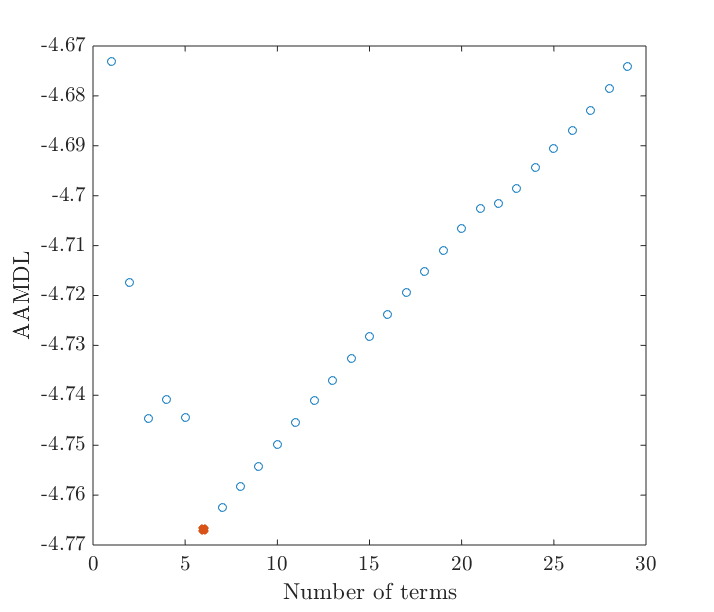
\includegraphics[width=\linewidth]{Figures/example_figure.png}
	\caption{Example of a png file. To preserve the ratio, set width to linewidth.}\label{fig:example}
\end{figure}
\par An example of pseudocode is demonstrated in Algorithm \ref{alg:kf}.

%------------------------------------------------
\begin{algorithm}[!t]
	\caption{Kalman filter}\label{alg:kf}
	\begin{algorithmic}[1]
		\renewcommand{\algorithmicrequire}{\textbf{Input:}}
		\renewcommand{\algorithmicensure}{\textbf{Output:}}
		\REQUIRE Measurement vector $\mathbf{y}_{1:\T}$; model matrices; state noise variance, $Q_{\td}$; measurement noise variance, $R_{\td}$; initial state estimate, $\bar{\mathbfit{x}}_0$; and initial covariance, $\mathbfit{P}_0$.
		\ENSURE Sequence of filtered state estimates, $\{\hat{\mathbfit{x}}_{\td \mid \td}\}^{\T}_{\td = 0}$; filtered covariances, $\{\mathbfit{P}_{\td \mid \td}\}^{\T}_{\td = 0}$.
		\FOR {$\td \gets 1,\T$}
		\STATE Compute prior state estimate $
		\hat{\mathbfit{x}}_{\td \mid \td-1} = A_{\td} \hat{\mathbfit{x}}_{\td-1 \mid \td-1} + B_{\td} \mathbfit{u}_{\td}$; \\	
		\STATE Compute prior covariance $
		\mathbfit{P}_{\td \mid \td-1} = A_{\td} \mathbfit{P}_{\td-1 \mid \td-1} A_{\td}^{\top} + Q_{\td}$;\\
		\STATE Compute residual $\tilde{\mathbfit{y}}_{\td} =\mathbfit{y}_{\td} - C_{\td} \hat{\mathbfit{x}}_{\td \mid \td-1}$; \\
		\STATE Compute residual covariance $ \mathbfit{S}_{\td \mid \td} = C_{\td} \mathbfit{P}_{\td \mid \td-1} C_{\td}^{\top} + R_{\td}.$; \\
		\STATE Compute Kalman gain $K_{\td} = \mathbfit{P}_{\td \mid \td-1} C_{\td}^{\top}\left(\mathbfit{S}_{\td \mid \td}\right)^{-1}$; \\
		\STATE Compute posterior state estimate $\hat{\mathbfit{x}}_{\td \mid \td1} = \hat{\mathbfit{x}}_{\td \mid \td-1}  + K_{\td} \tilde{\mathbfit{y}}_{\td}$; \\
		\STATE Compute posterior covariance $\mathbfit{P}_{\td \mid \td} = \mathbfit{P}_{\td \mid \td-1} - K_{\td}\mathbfit{S}_{\td \mid \td}K_{\td}^{\top}$; \\			
		\ENDFOR
	\end{algorithmic}
\end{algorithm}
\section{Results}

\begin{table*}[t]
	\centering
	\caption{Example of page-wide figure table}
	\centering
	\begin{tabular}{rrrrrrrr}
Step & Terms & C1 & C2 & C4 & C5 & C6 & AEER($\%$) \\ 
\hline 
1 & $x_4 x_4$ & -26.04 & -20.99 & -10.69 & -10.96 & -191.78 & 89.511 \\ 
2 & $x_3$ & 75.42 & 59.58 & 33 & 26.06 & 508.94  & 8.849 \\ 
3 & $x_1 x_4$ & 0.62 & 0.76 & 0.32 & 0.48 & 8.55 &  0.139 \\ 
4 & $x_1 x_1$ & 0.01 & -0.19 & -0.15 & -0.22 & 0.05 &  0.045 \\ 
5 & $x_2$ & 0.71 & -0.73 & -2.24 & -0.66 & 45.94 &  0.032 \\ 
6 & $x_4$ & -171.24 & -139.22 & -69.61 & -73.69 & -1273.02 & 0.006 \\ 
7 & $c$ & -233.16 & -200.83 & -93.74 & -119.7 & -1805.9 &  0.308 \\ 
8 & $x_3 x_4$ & 15.47 & 12.1 & 6.36 & 5.68 & 110.13 &  0.093 \\ 
\hline 
\end{tabular}
\end{table*}

\par \blindtext % Dummy text



\par \blindtext % Dummy text

%------------------------------------------------

\section{Discussion}

\subsection{Subsection One}
\par \blindtext % Dummy text
A statement requiring citation \cite{Wei2008}
\par \blindtext % Dummy text
\subsection{Subsection Two}
\par \blindtext % Dummy text
\par Figure \ref{fig:tikz} demonstrates embedding tikz files.
\par \blindtext % Dummy text
\begin{figure}[!t]
	\centering
	\definecolor{mycolor1}{rgb}{0.00000,0.44700,0.74100}%
	\definecolor{mycolor2}{rgb}{0.85000,0.32500,0.09800}%
	% This file was created by matlab2tikz.
% Minimal pgfplots version: 1.3
%
\definecolor{mycolor1}{rgb}{0.00000,0.44700,0.74100}%
\definecolor{mycolor2}{rgb}{0.85000,0.32500,0.09800}%
%
\begin{tikzpicture}

\begin{axis}[%
width=6cm,
height=4cm,
at={(0cm,0cm)},
scale only axis,
xmin=1,
xmax=15,
xlabel={Number of terms},
ymin=-3.2,
ymax=-2,
ylabel={AAMDL},
legend style={legend cell align=left,align=left,draw=white!15!black}
]
\addplot [color=mycolor1,only marks,mark=o,mark options={solid},forget plot]
  table[row sep=crcr]{%
1	-2.11570305645112\\
2	-2.79305839626823\\
3	-2.82935915360095\\
4	-2.83995463691255\\
5	-2.84820086237127\\
6	-2.84802935769127\\
7	-2.95749685829162\\
8	-3.00104696019893\\
9	-3.00045381599073\\
10	-3.00058067310023\\
11	-2.99929045654952\\
12	-2.99893492528062\\
13	-2.99723787908848\\
14	-2.99552868329925\\
15	-2.99382083512231\\
};
\addplot [color=mycolor2,line width=5.0pt,only marks,mark=asterisk,mark options={solid},forget plot]
  table[row sep=crcr]{%
8	-3.00104696019893\\
};\label{tikz:point}
\end{axis}
\end{tikzpicture}%
	\caption{Example of a tikz figure. Refererence to the plot in the figure (\ref{tikz:point}).}\label{fig:tikz}
\end{figure}
%----------------------------------------------------------------------------------------
%	REFERENCE LIST
%----------------------------------------------------------------------------------------
\section{Conclusion}
\blindtext

\printbibliography

%----------------------------------------------------------------------------------------

\end{document}
